\ifdefined\THESIS
    \chapter{\uppercase{Analysis of Distance to Contacts}}
\else
    \section{Analysis of Distance to Contacts}
    \label{sec:analysis}
\fi

% FIXME: For each subsection finding (e.g., "What is the distribution of
% contacts?") you need to add more intuition/analysis. Walk the reader through
% each figure. Highlight some actual numbers from the figures in the text. Tell
% us what those numbers mean. Tell me what I should learn. You do some of this
% already, but it really needs to be expanded. Remember, your reader is not as
% on top of this material as you are, so you need to do more handholding.

% FIXME: For all figs, you might want to add a takeaway sentence in the
% caption. So if a reader only looks at the fig (without following along in the
% text), they can learn something.

Every user who has multiple contacts will have some contacts who are much
closer than others.
%
In order to estimate the locations of users, we would like
to find out which users are most likely to live nearby.
%
In this section, we investigate how various types of contacts correlate with
proximity.
%
All of the analysis in this section was done on the contacts of the 249584
geo-located users.
%
Contacts with a predicted location error that was greater than or equal to 1000
miles were filtered out.

\begin{figure}[tb]
\centering
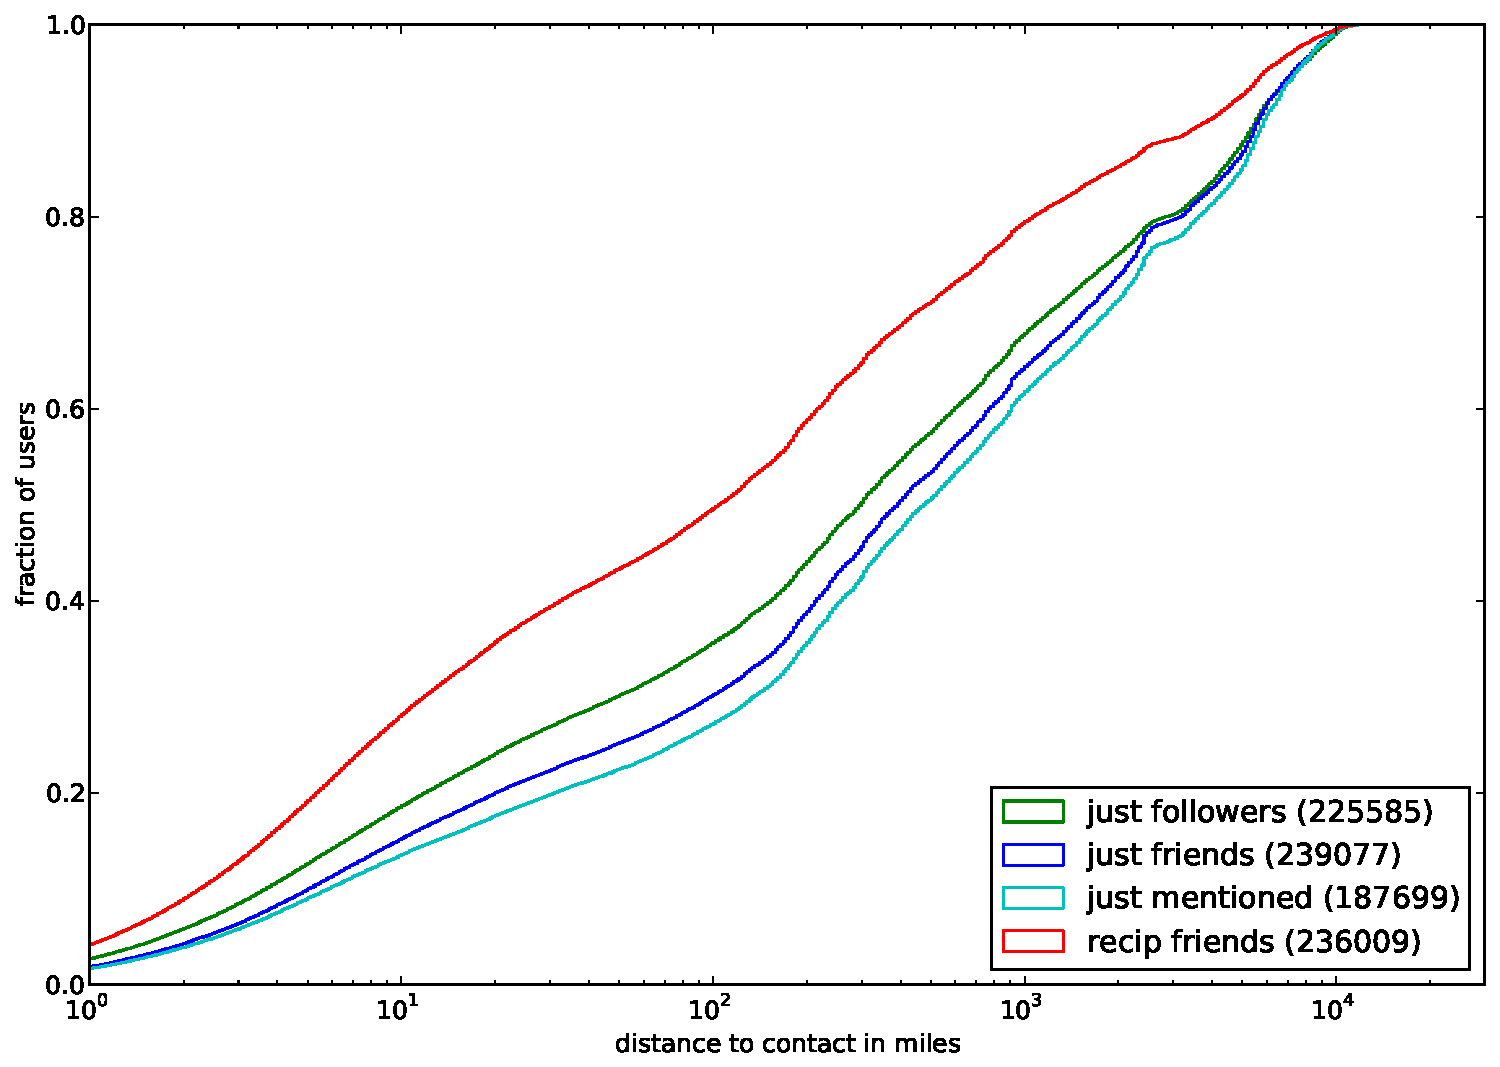
\includegraphics[width=\linewidth]{figures/edge_types_cuml.pdf}
\caption{
CDF of distance from geo-located users to users they have some contact
with.
%
Reciprocal friends tend to be closer than other types of friendships.
}
\label{fig:EdgeTypesCuml}
\end{figure}

\subsection{What type of contact is closest?}
\label{sec:EdgeTypes}

Figure~\ref{fig:EdgeTypesCuml} shows the cumulative distribution
function(CDF) of the distance between a geo-located user and several types of
contacts.
%
Distance is plotted on a logarithmic scale to show both local and
global effects.
%
On a logarithmic scale, the contacts are fairly evenly distributed from being
nearby to being on the opposite side of the world.
%
For reciprocal friends, the 1\textsuperscript{st} quartile, median, and
3\textsuperscript{rd} of the distances are 7.9 miles, 106 miles, and 720 miles
respectively.
%
There is a relatively flat section in all the lines around 3,000 miles.
%
3,000 miles is longer than the distance between the east coast of the U.S. and
the west coast, but shorter than the distance from the east coast of the U.S.
to Europe, so there are few population centers that are this distance apart.

In general, reciprocal friends are the closest, followed by followers, friends,
and finally users who are just mentioned.
%
38\% of reciprocal friends live within 25 miles while only 18\% of users
who are just mentioned live within that radius.
%
While it may seem that since being followed by someone and following someone
should be identical, they are not.
%
Celebrity and news accounts on Twitter often have large numbers of followers,
but they normally do not follow a large number of users.
%
Since the geo-located user was selected randomly, they are usually an average
user and not a celebrity.
%
If they follow someone, it might be a celebrity; however, if someone follows
them, it is probably someone who knows them.

\begin{figure}[tb]
\centering
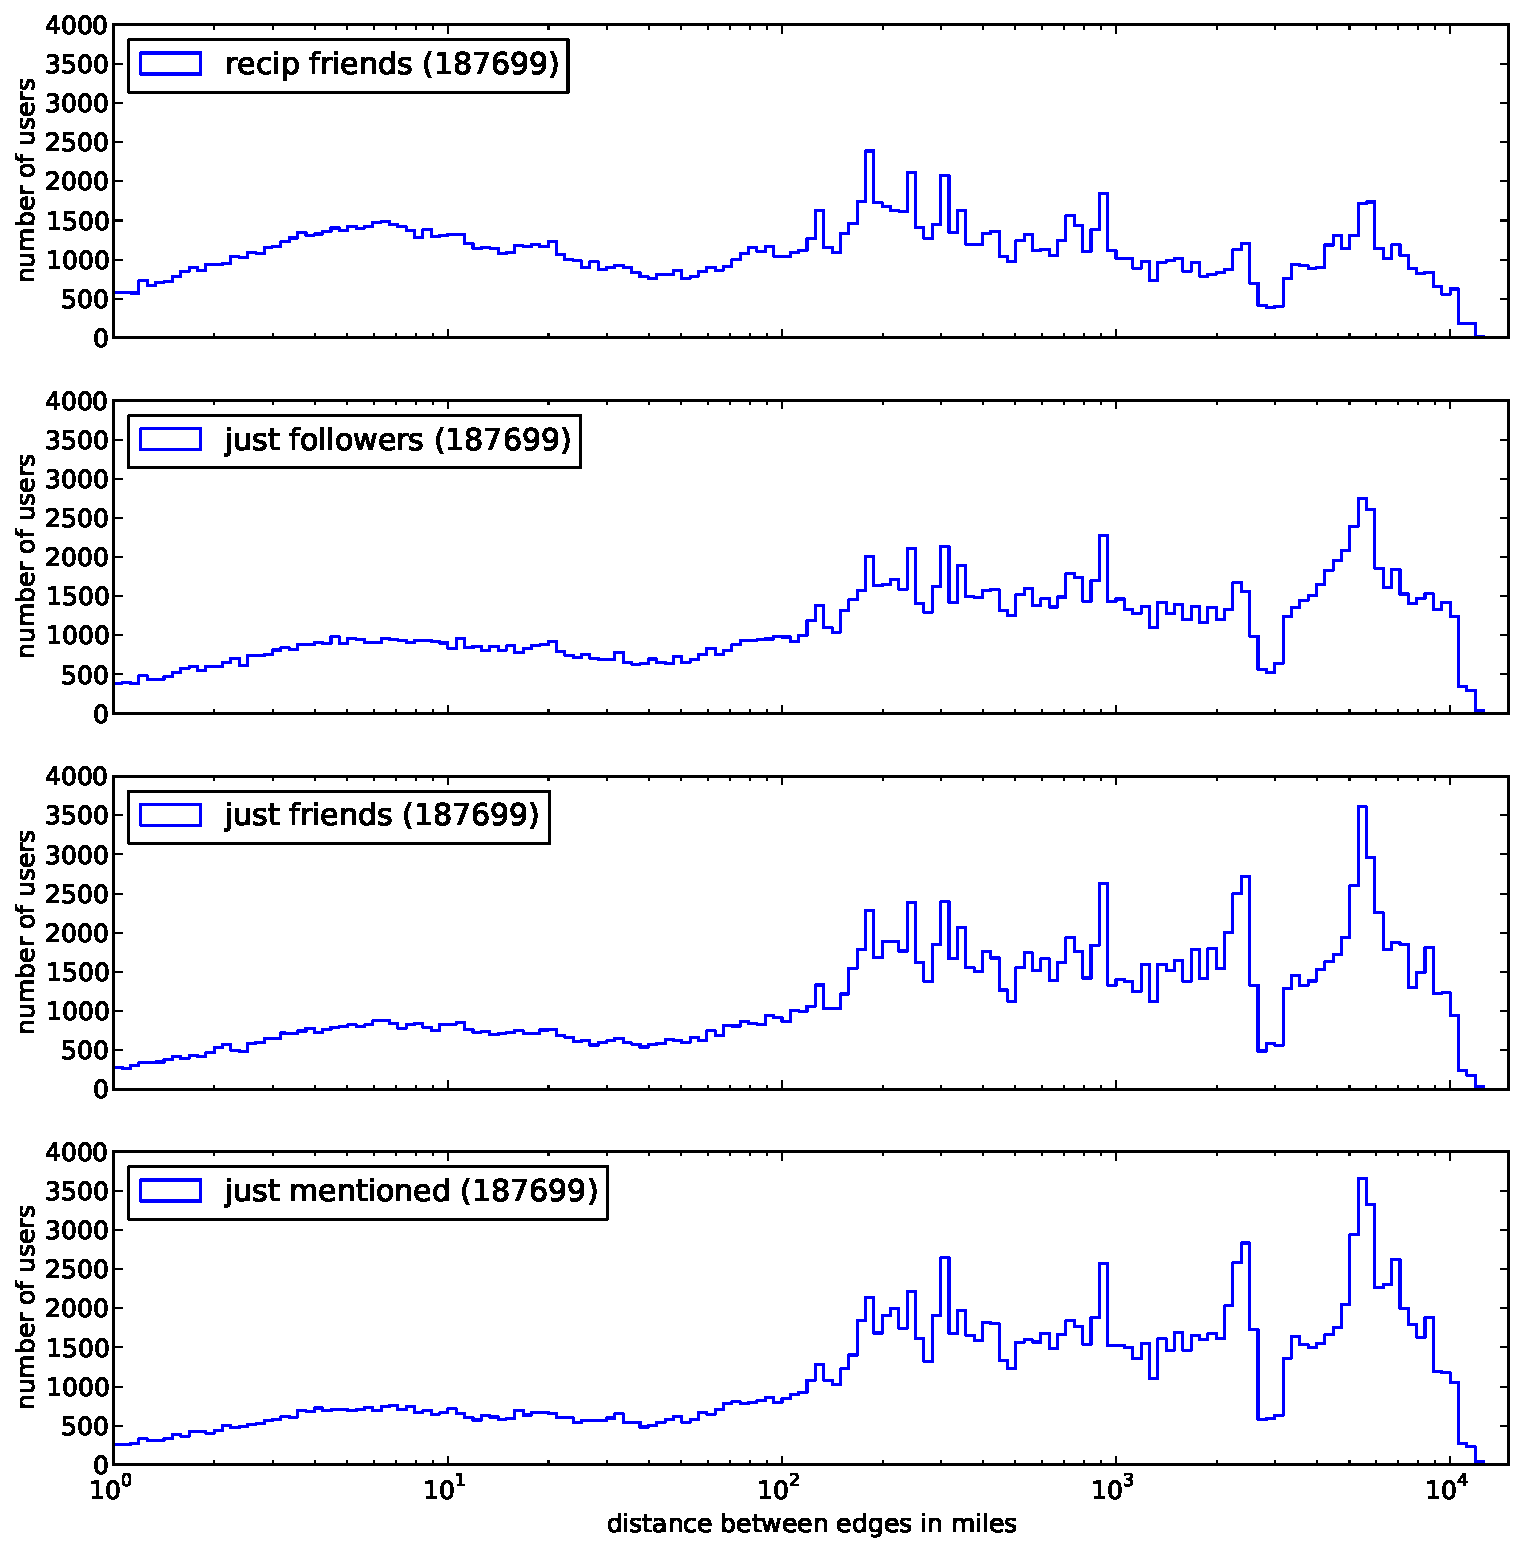
\includegraphics[width=\linewidth]{figures/edge_types_norm.pdf}
\caption{
Histogram of distance to users for different types of relationships.
The curves in this figure are the derivatives of the curves in
Figure~\ref{fig:EdgeTypesCuml}.
}
\label{fig:EdgeTypes}
\end{figure}

\subsection{What is the distribution of contacts?}

To understand the distribution of contacts, we created a histogram of the distances between various types of contacts.
We sorted the distances to contacts into 160 logarithmically
scaled bins (40 bins for each power of 10).
%
Figure~\ref{fig:EdgeTypes} shows the result of plotting the histogram.
%
All four types of contacts follow roughly the same
distribution: one peak around 10 miles from people who live nearby, and several
other peeks between 100 and 10,000 miles.
%
These peeks occur at the distances between major population centers.

There is a local maximum in all the graphs at around 8 miles.
%
Since the contacts often list the name of their town, there is a small distance
between the geocoded location of the town and the location of the geo-located
user's tweets.
%
There aren't as many contacts in the 30 to 150 mile range, but then after 150
miles, peaks start appearing for major cities.
%
One reasonable explanation for this is that Twitter is not just a social
network; it is also a news distribution network as described in
\cite{kwak2010why}.
This distribution suggests that users have two types of contacts: people who
they met in real life, and people who they met online or know about via
mainstream media.
%
The former group is useful for predicting location and the latter group is not.
%
In section~\ref{sec:model}, we use this idea that there are two types of
contacts to build a predictive location model based on social ties.


\begin{figure*}[tb]
\centering
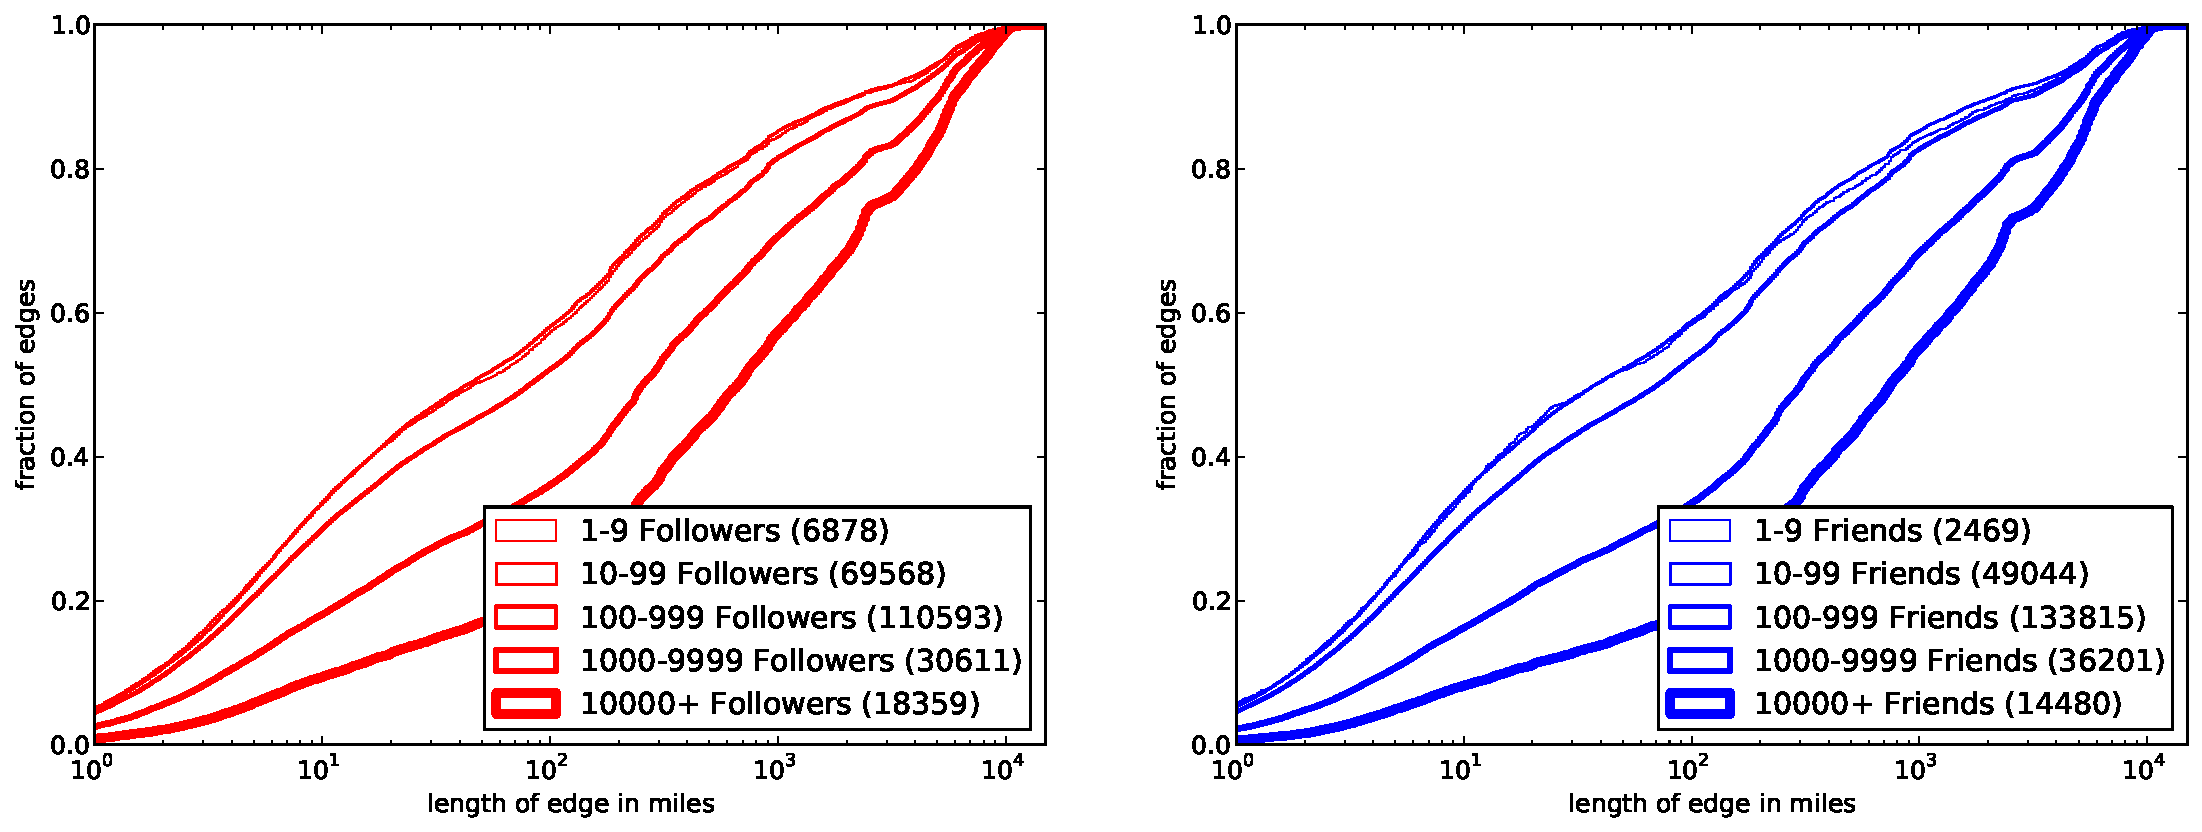
\includegraphics[width=\linewidth]{figures/edge_counts.pdf}
\caption{
A comparison between number of followers and proximity---people who have more
friends or followers tend to be further away.
}
\label{fig:EdgeCounts}
\end{figure*}

\subsection{Does the number of friends and followers a person have affect how
close they are?}

Since the primary goal of this research is to predict the location of users, we
focus our attention on the number of friends and followers a contact has rather
than the numbers for the geo-located user.
%
We took each of the reciprocal friendships what we looked at in
Section~\ref{sec:EdgeTypes} and put them into log-scaled bins based on their
number of friends or followers that the contact had.
%
Figure~\ref{fig:EdgeCounts} shows the result of this procedure.

In general, people who are more promiscuous followers and friends are less
likely to live nearby.
%
This makes sense because it is easy to meet 15 Twitter users in real life, but
very few people know 1000 Twitter users who live in the same town.
%
Contacts with 10--99 followers were within 25 miles of their geo-loacted friend
45\% of the time while contacts with 1000--9999 followers were nearby only 26\%
of the time.
%
There was a similar result in the number of friends: the prorportion of local
contacts went from 46\% down to 23\%.

Mainstream media and celebrity accounts such as the New York Times and Lady
Gaga have millions of followers while normal users rarely have more than a few
hundred.
%
Follower count and friend count are good ways to distinguish celebrity and news
accounts which are useless for location prediction.

aoeu aoeu.

\ifdefined\THESIS
    \begin{figure*}[tb]
    \centering
    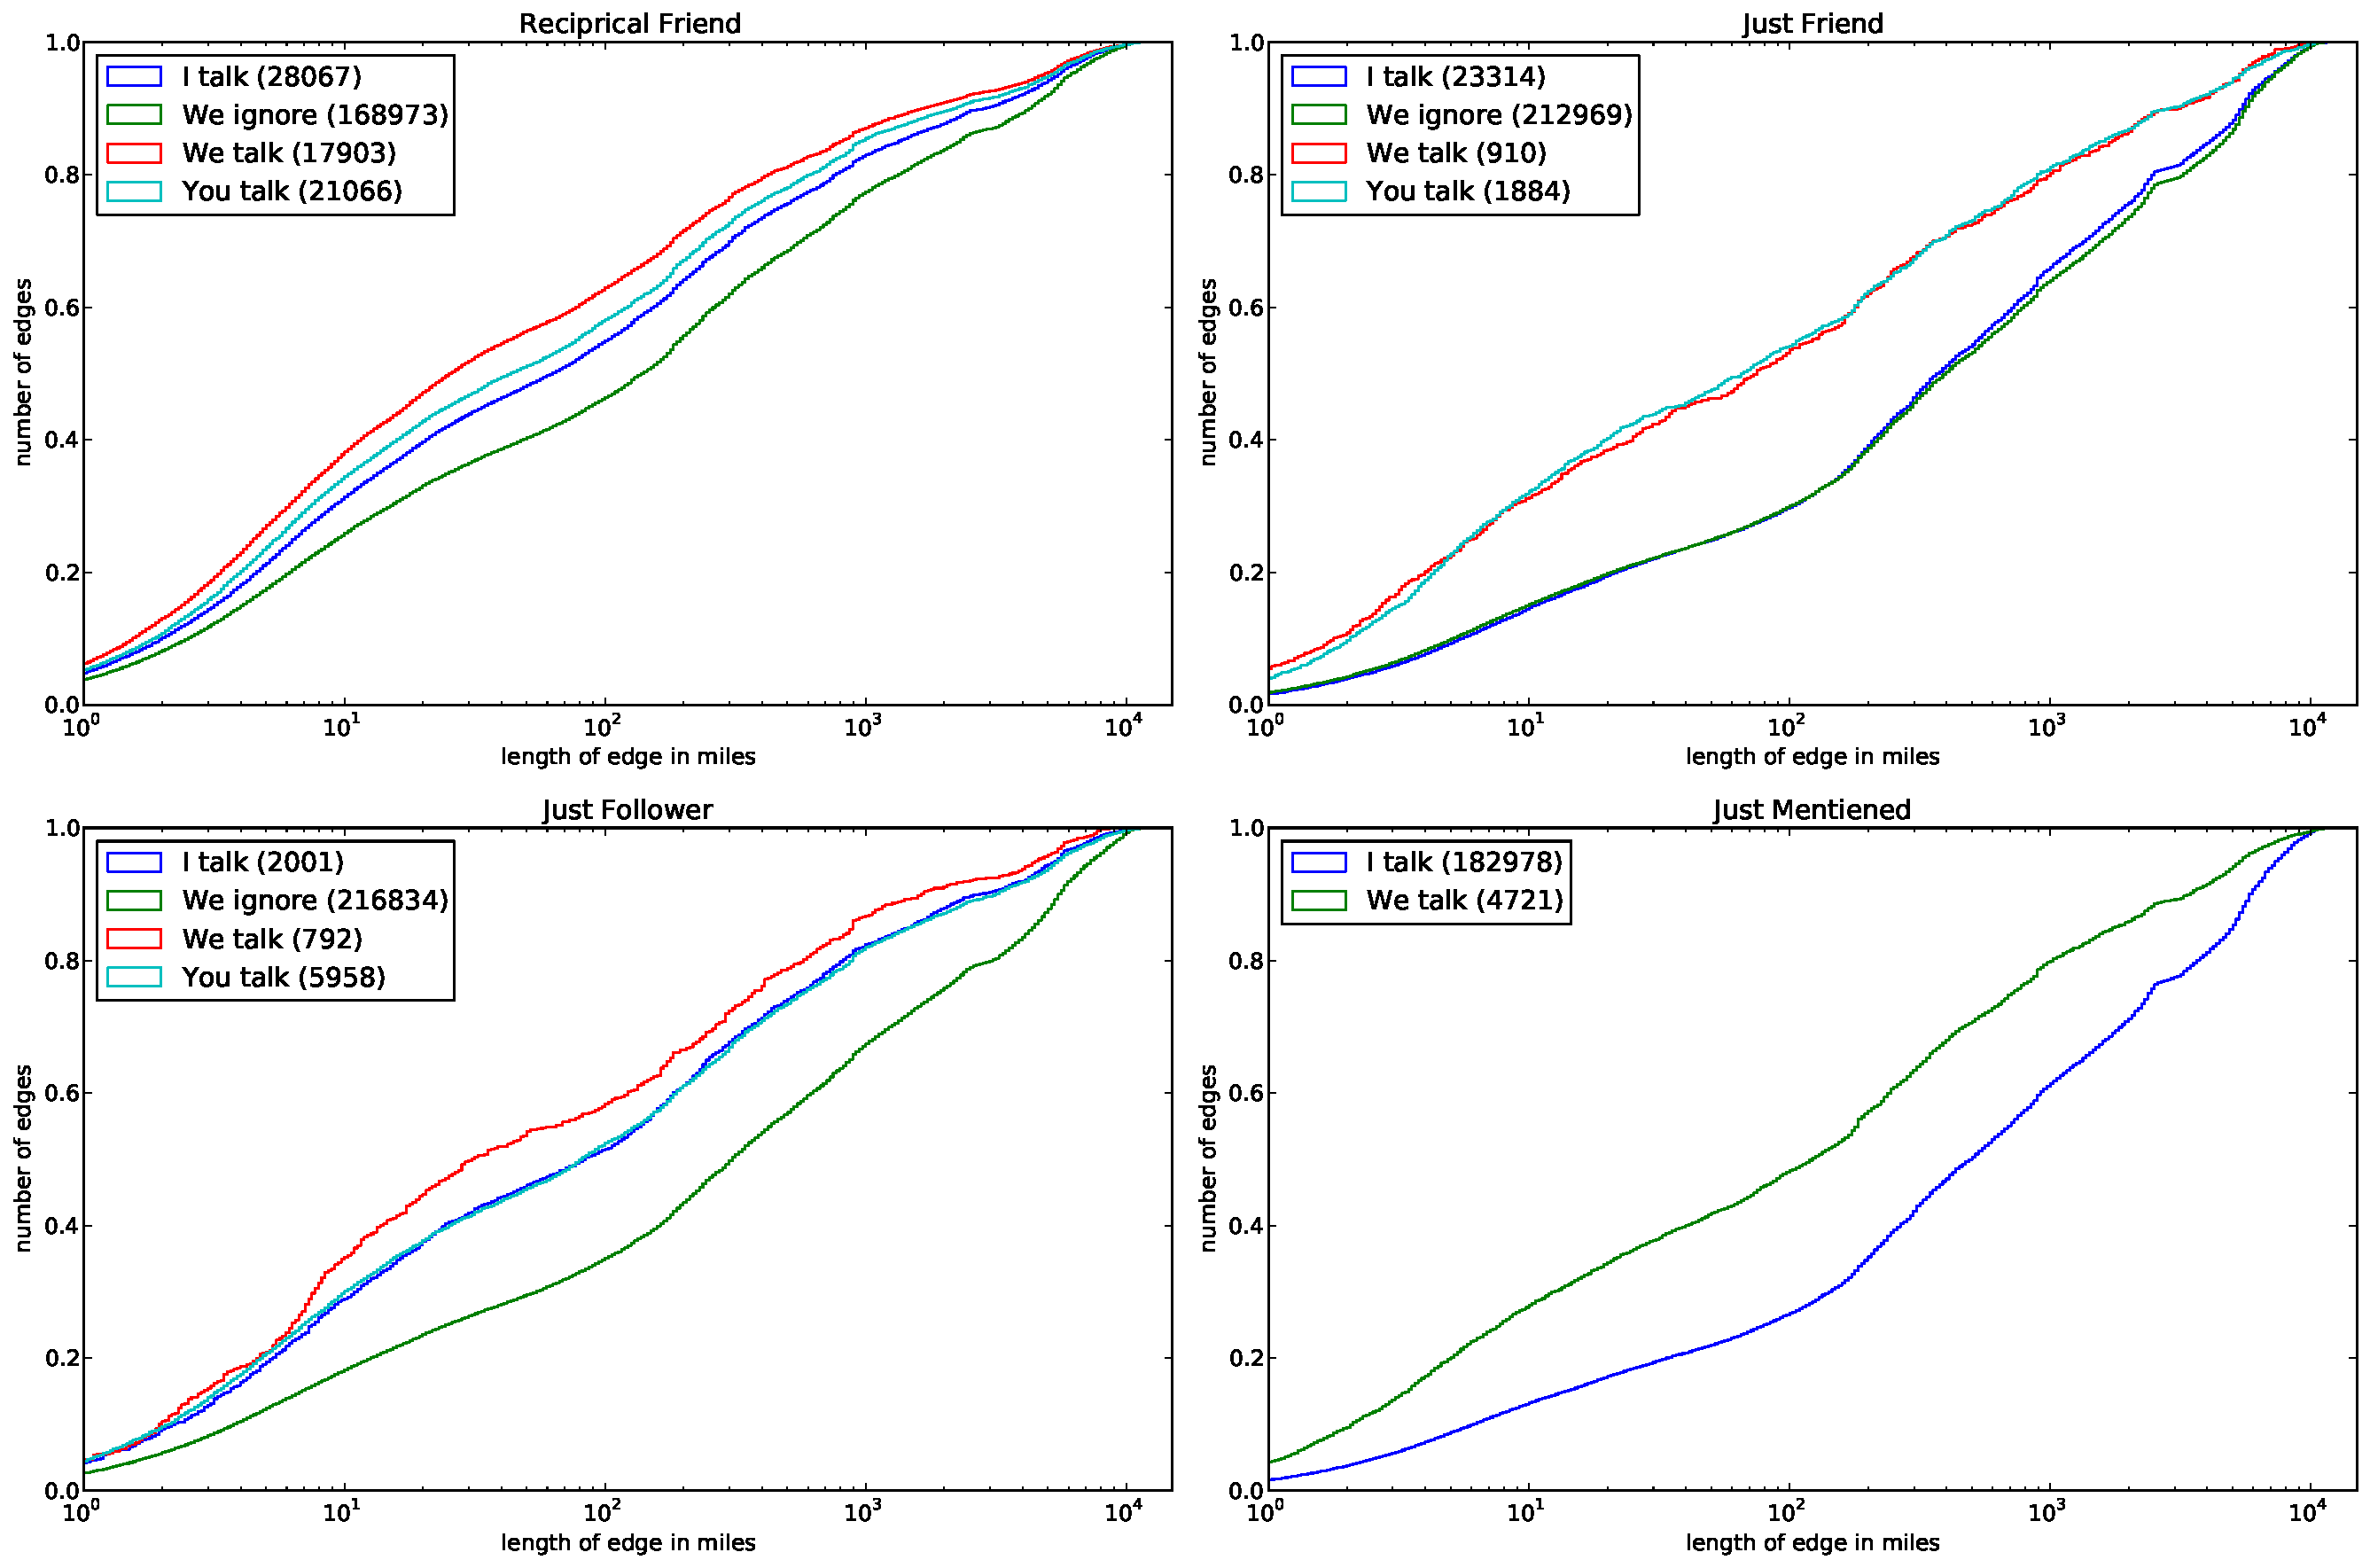
\includegraphics[width=\linewidth]{figures/com_types.pdf}
    \caption{
    CDF of the distance between a geo-located user and various types of contacts
    piloted on a logarithmic scale.
    }
    \label{fig:ComTypes}
    \end{figure*}
\fi


\begin{table*}[tb]
\centering
\begin{tabular}{l | r r | r r | r r | r r | r r}
    & \multicolumn{2}{|c}{both mention}
    & \multicolumn{2}{|c}{target mentions}
    & \multicolumn{2}{|c}{contact mentions}
    & \multicolumn{2}{|c}{both ignore}
    & \multicolumn{2}{|c}{overall} \\
    \cline{2-11}
    &local&count&local&count&local&count&local&count&local&count \\
    \hline
    Recip Friend & 42\%&28067 & 50\%&17903 & 45\%&21066 & 35\%&168973 & 38\%&236009 \\
    Just Follower & 40\%&2001 & 47\%&792 & 40\%&5958 & 25\%&216834 & 25\%&225585 \\
    Just Friend & 21\%&23314 & 40\%&910 & 42\%&1884 & 21\%&212969 & 21\%&239007 \\
    Just Mentioned & 18\%&182978 & 36\%&4721 & & 0 & & 0 & 18\%&187699 \\
\end{tabular}
\caption{
If geo-located users interact with their contacts, then they are more likely to
live nearby.
%
In this table, ``I'' refers to the geo-located user. ``You'' refers to their
contact.
%
\emph{Should I highlight cells in the table?, Should I color-code?}
}
\label{tab:ComTypes}
\end{table*}

\subsection{Are users closer to people they communicate with?}

We looked at the 100 most recent tweets for the geo-located users and one of
each type of their contacts.
%
The edges were divided into groups based on whether the geo-located user
mentioned the contact and whether the contact mentioned the geo-located user.
%
For each of the groups, we calculated the the percentage of contacts who are
live within 25 miles of the targets and the number of edges in that group.
%
This is shown in Table~\ref{tab:ComTypes}.
%
Since contacts who were just mentioned were mentioned by the geo-located
user by definition, the contact mentions and both ignore table cells are
empty.

In almost every case, increased communication increases the probability that
two users live near each other.
%
There is one exception: when an average user mentions someone they follow who
does not follow them back, it has no effect---in both cases the contact is
local 25\% of the time.
%
In other words, if a random user mentions a celebrity who does not bother to
reply, they probably do not live in the same area.
%
On the other hand, in the rare event that someone who is just a friend replies
to their follower, then the probability that they live near each other is much
higher--it goes from 21\% to 42\%.

The weakest type of contact is for users who were just mentioned, but never
replied to.
%
If the person is mentioned, then 36\% of users with no
friend/follow relationship who have a conversation live within 25 miles.
%
This is approximately equal to the 35\% of reciprocal friends who ignore each
other and live within 25 miles.
%
Unsurprisingly, the strongest type of connection is reciprocal friends who
communicate.
%
One challenge to using communication patterns as a source of information for
location prediction is that the communication patterns that are correlated
with proximity are rare.

\begin{table}[tbh]
\centering
\begin{tabular}{l | r r | r r}
    & \multicolumn{2}{c}{Public}
    & \multicolumn{2}{|c}{Private} \\
    \cline{2-5}
    &local&count&local&count \\
    \hline
    Recip Friend & 37\%&211136 & 41\%&24873 \\
    Just Follower & 25\%&204417 & 31\%&21168 \\
    Just Friend & 21\%&233849 & 39\%&5228 \\
    Just Mentioned & 18\%&183368 & 35\%&4331 \\
\end{tabular}
\caption{
    Comparison between public accounts and private accounts on Twitter.
    Private accounts tend to be closer.
}
\label{tab:EdgeTypesProt}
\end{table}

\subsection{Are users closer to private accounts?}

Like many social networks, Twitter allows users to control the privacy settings
on their account.
%
The specifics differ from network to network, but in Twitter's case
a user can make their account private which means followers have to get
permission to follow the account.
%
There are demographic differences between public and protected accounts.
%
For example, Gilbert \cite{gilbert2008network} demonstrates that rural users
are more likely to make their accounts private than public accounts.
%
In the case of protected accounts on Twitter, basic information
about their profile such as their location and the number of friends and
followers is public, but their friends list, followers list, and the text of
their tweets is private, and not available for analysis.

As seen in Table~\ref{tab:EdgeTypesProt}, the most dramatic difference between
private and public occurs if a user follows a protected account.
%
Since users generally only allow people they know to follow a protected
account, this brings the users almost as close together as if they were
reciprocal friends.
%
On the other hand, if a protected account follows the geo-located user, they
are only slightly more likely to be nearby.

\begin{figure}[tb]
\centering
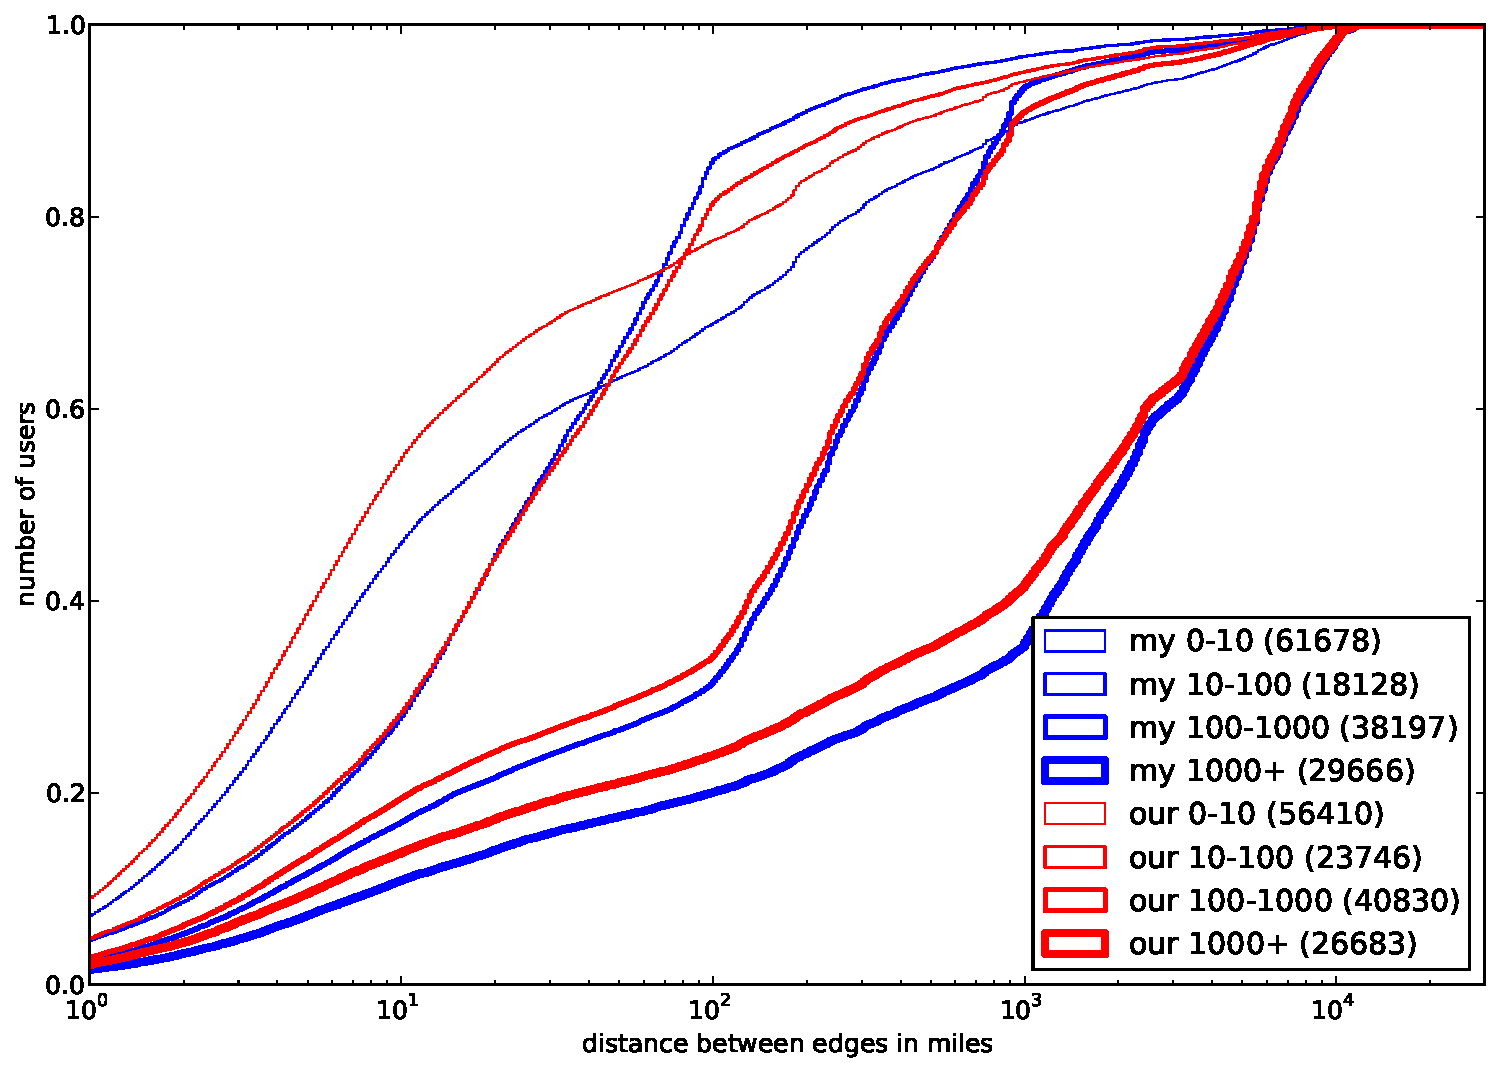
\includegraphics[width=\linewidth]{figures/near_triads.pdf}
\caption{
Comparison between distance to a mutual friend, labeled ``our'', and someone
who is not a mutual friend, labeled ``my''.
If two contacts are mutual friends and live near each other, a target user is
more likely to live near them than two contacts who live nearby but are not
mutual friends.
}
\label{fig:NearTriads}
\end{figure}

\subsection{If two of your friends live near each other, does that increase the
chance that they live near you?}

In this section, we turn our attention to triangles of users.
Finding useful relationships between the edges of a social triangle is tricky
because the three distances depend on each other.
Unfortunately, it is fairly simple to show using the triangle inequality theorem
that if two users are 1000 miles apart, then the third member of the triangle
has to be at least 500 miles from one of the other two.
Since this isn't a useful result, we designed a more complex experiment to
analyze the relationship between the sides of the triangle.
A script searched for a specific pattern in the social network of
the target user's reciprocal friends: two people who were friends with each
other and a third person who had no connection with the other two:

\begin{center}
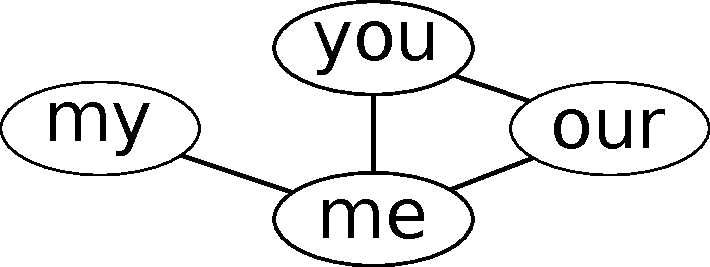
\includegraphics[width=0.3\linewidth]{figures/near_triads_dia.pdf}
\end{center}

To help label the four users, we describe this social graph from the
perspective of the target user:

\begin{itemize}
\item ``me'' is the target user
\item ``you'' is the contact who is reciprocal friends with ``me''
\item ``my'' has no relationship with ``you'' and is reciprocal friends with ``me''
\item ``our'' is reciprocal friends with both ``me'' and ``you''
\end{itemize}

We found this pattern for 147669 of the geo-located users.
%
If a user had multiple instances of this pattern, it picked one of them
randomly so that particular users would not bias the results.
%
Since our crawler only retrieved friend and follower information for a few
reciprocal friends per user, it is reasonable to assume that this pattern
is much more common, but the sample is more than enough data to draw some
conclusions.

Figure~\ref{fig:NearTriads} shows a comparison between distances to the ``my''
users and the ``our'' users.
%
For each of the ``my'' users and the ``our'' users, we put them into one of
four logarithmically scaled bins based on their distance from the ``you'' user.
%
Then we plot the CDF for the distance from the target to the ``my'' and ``our'' users.
%
This allows us to investigate the effect of mutual friendship on distance.
We report one very simple result: if two of your friends are close (within 10
miles), then whether they know each other or not is strongly affects how close
you are to them.
%
If they are farther apart, it doesn't matter.

\begin{figure}[tb]
\centering
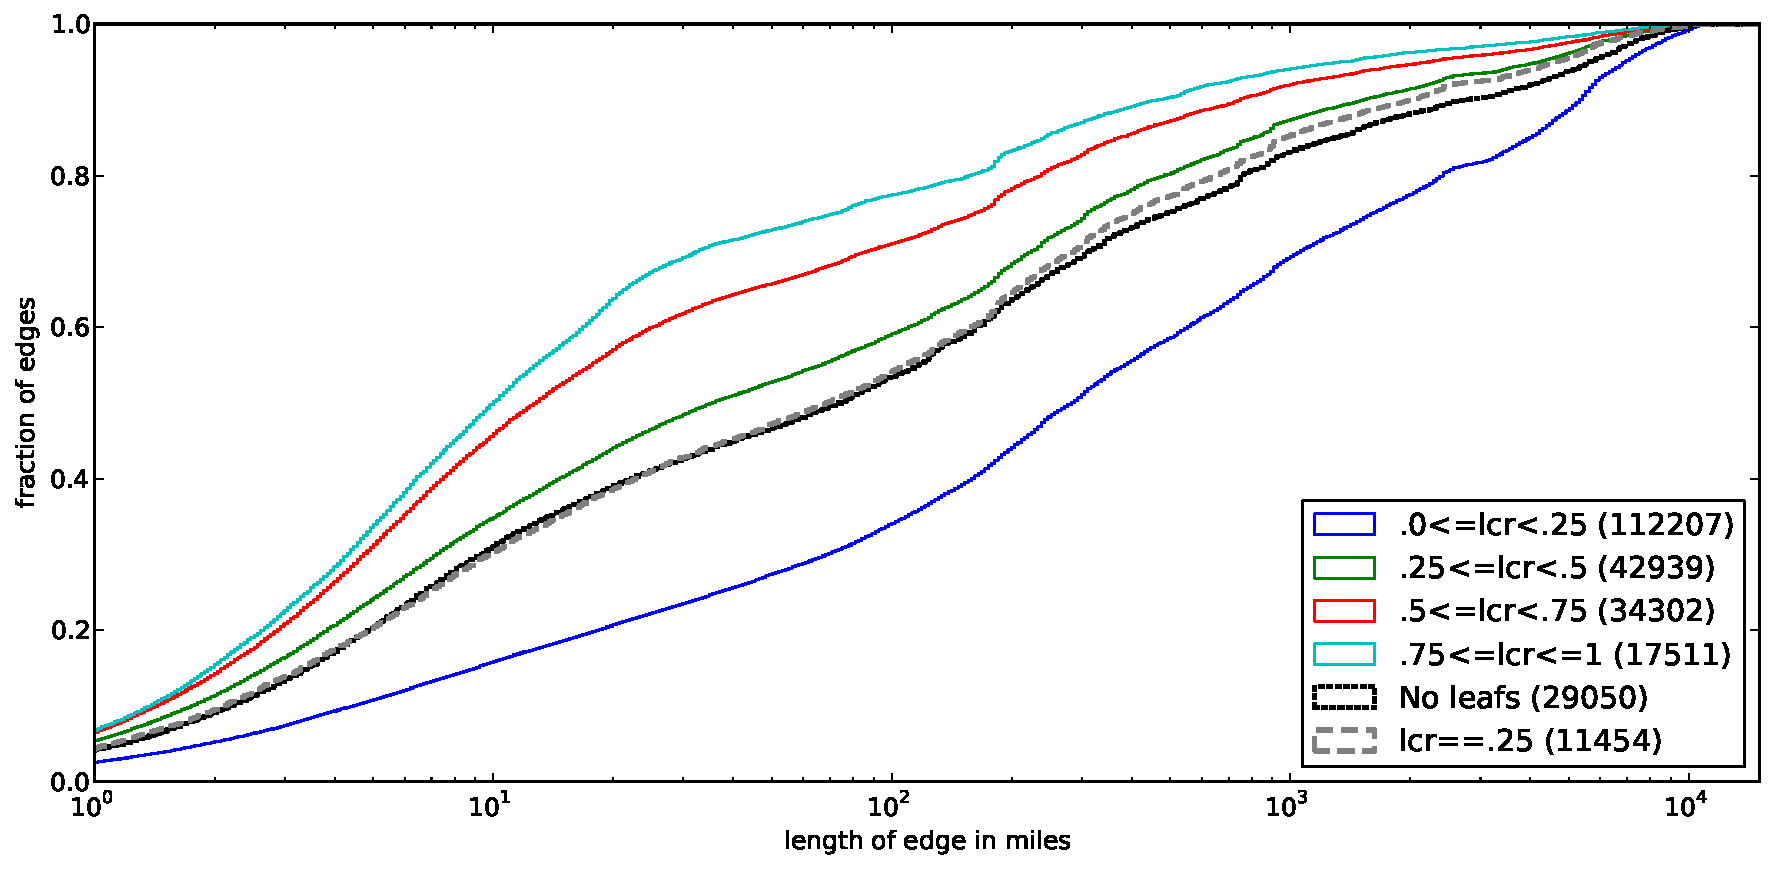
\includegraphics[width=\linewidth]{figures/locals_10.pdf}
\caption{
The colored lines show the distance to contacts split into groups based on the
proportion of the contact's friends and followers who live near the contact.
The dotted line shows the distance to contacts who have no locatable contacts.
This graph is based on at most 10 leafs per contact.
Contacts who have a high proportion of nearby leafs are much more likely to
live near the target user.
}
\label{fig:Local10}
\end{figure}

\begin{figure}[tb]
\centering
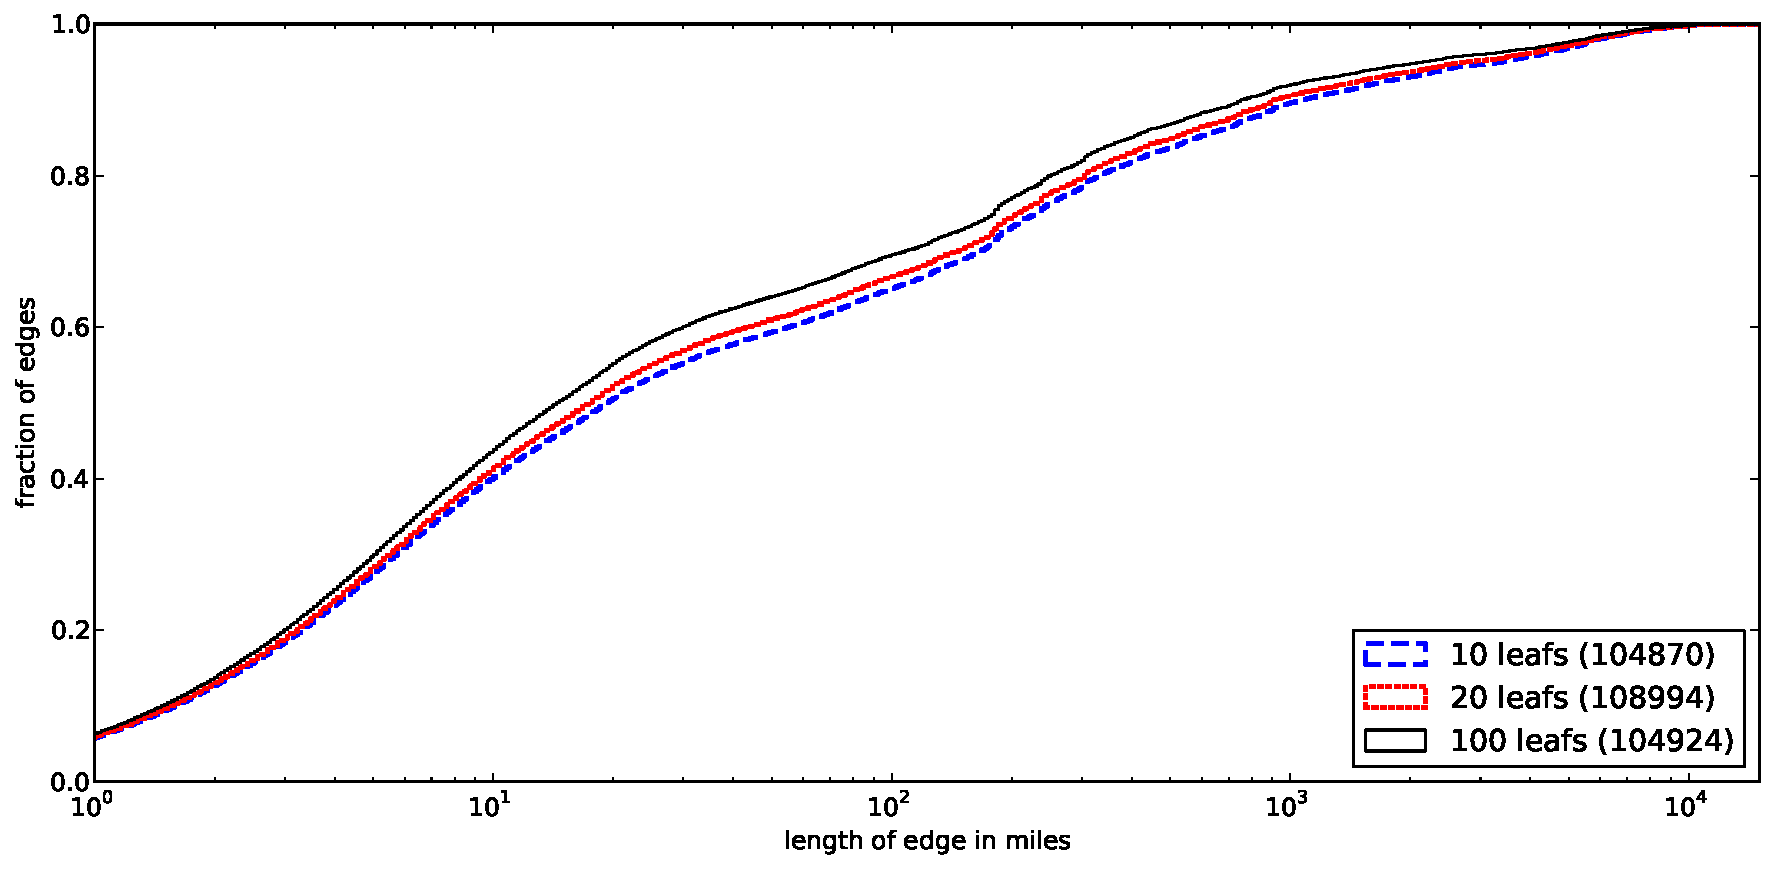
\includegraphics[width=\linewidth]{figures/locals_cmp.pdf}
\caption{
    Distances to contacts with a local contact ratio better than the median LCR
    for several numbers of leafs.
    Although looking at more leafs makes users with a high LCR more likely to
    be nearby, it probably doesn't justify how long it takes.
}
\label{fig:LocalCmp}
\end{figure}

\subsection{Are some users closer to all of their friends and followers?}
\label{sec:closer}

In the previous sections we only looked at the contacts of the geo-located
users.
%
In this section we will go two steps out on the social graph and
investigate the friends-of-friends.
%
We want to know if some users are more localized than others.

\textbf{Local Contact Ratio}(LCR) is the fraction of a user's followers who live
within 25 miles of the contact.
%
Around one in ten contacts did not have any followers with a location--they were
treated as a separate group.
%
We repeated this procedure on the contacts' friends to produce
Figure~\ref{fig:EdgeCounts}.

\emph{Here's my formula, math me, maybe?}

In \cite{li2012towards}, the authors model the probability distribution of
user's followers using a gaussian distribution, and use this to build a
location prediction system.
%
There are many other ways to analyze the leafs: average distance to the leafs,
median distance to the leafs, fitting the distances to a curve such as a
gaussian.
%
We are looking at location prediction anywhere in the world, which means
contacts may be 10,000 miles away, and a location 10,000 miles away is nearly
as bad as a loctation 1000 miles away.

The figure shows that some users are much more local than other users.
For example, a local newspaper may have thousands of followers and few friends,
but the people who follow a newspaper are generally local.
According to the other factors we looked at, the newspaper is a bad predictor
of location, but in reality it is a great predictor.

Of the factors we have investigated, this is the most strongly correlated with
distance.
\emph{Can you prove this?}
One problem with this technique is that it is somewhat expensive to deal with
the large number of profiles two steps out on the social graph.
%
Our crawler originally looked at 100 leafs per contact because Twitter's API
will return up to 100 profiles at a time, but .
%
In Figure~\ref{fig:LocalCmp}, we compare contacts with a high LCR calculated
using at most 100 leafs per contact to at most 10 leafs per contact.
%
The percentage of contacts within 25 miles with a good LCR based on 10 leafs,
20 leafs, and 100 leafs was 53\%, 55\%, and 58\%, respectively.
%
All of these are noticably closer than reciprocal friends who are within 25
miles 38\% of the time.


